\section{Step 1 -- getting the cross}
This step will get the first layer cross, this equals fitting and orientating of the edges in the yellow face. 
The step is generally described in subsection \ref{sub:step1}.
The first question our program needs to ask is whether the edge \cpiece{}s already are positioned correctly. If that is the case and the edge \cpiece{} is also oriented correctly, the program proceeds to the next edge \cpiece{}. If not, an algorithm is performed, which changes the edge piece's orientation without ruining other possibly correctly positioned edge \cpiece{}s. 
This algorithm is known as \textit{algorithm 1}. When the edge \cpiece{} is in the the correct position and has the correct orientation, the program moves on to another edge \cpiece{}. 

If the edge \cpiece{} in question is not in its correct position, the program needs to know where the edge is positioned. 
The way this is done is by first checking if the edge \cpiece{} is positioned in the first layer. 
If this is the case the edge \cpiece{} in question is moved to the opposite layer. 
If the edge \cpiece{} is not in the first layer it can either be in the opposite layer or in the second layer.
Is the edge \cpiece{}  positioned in the second layer an algorithm is performed which moves the edge \cpiece{}  to the white layer, which is the opposite of the layer in which we make the cross.

Now that the edge \cpiece{}  is in white layer it needs to be moved to the position directly above where it is correctly positioned. 
The program does this by \twist{}ing the up face once (known as an U \twist{}) and checks if the edge \cpiece{} is above it's correct position.
The edge piece is now positioned in two faces -- the white face and the face which has the same color as the edge  \cpiece{}'s second \facelet{} i.e. the face that is not yellow.
In order to position the edge \cpiece{} that face is twisted twice.
The edge \cpiece{}  is now in it's correct position, and if it is oriented correctly the program moves on to another edge  \cpiece{} .
If the edge \cpiece{} is oriented incorrectly \textit{algorithm 1} is performed. If more edge  \cpiece{}s needs to be positioned or oriented correctly the program will continue with the same method until the cross is finished in which case the program moves on to the next step. see \ref{fig:FlCrossFlow}.

\begin{figure}[htbp]
	\centering
		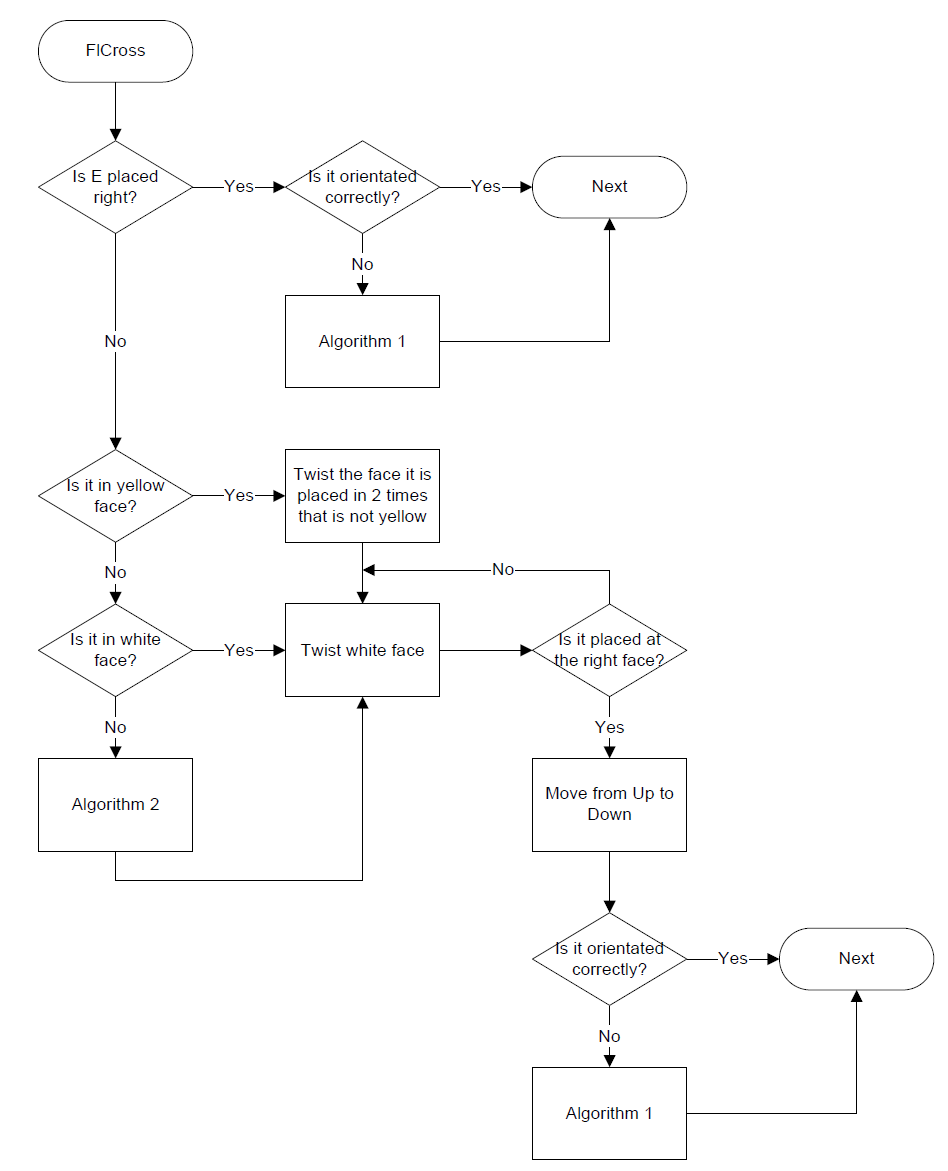
\includegraphics[scale=0.4]{input/pics/FlCrossFlow3.png}
	\caption{The picture illustrates what is done in step one.}
	\label{fig:FlCrossFlow}
\end{figure}
